% Practice Test 02 — Minnesota Edition
% Questions: 30 (22 MC + 8 SA)
% Generated by scripts/generate_practice_tests.py

\begin{practiceQuestion}{1-3-q30}{gsa}
\begin{questionText}
The table shows a proportional relationship between minutes and laps completed. Find $k$ and determine how many laps are completed in $15$ minutes.

\begin{center}
\begin{tabular}{|c|c|}
\hline
\textbf{Minutes ($x$)} & \textbf{Laps ($y$)} \\ \hline
$4$ & $3$ \\ \hline
$8$ & $6$ \\ \hline
$12$ & $9$ \\ \hline
$15$ & $?$ \\ \hline
\end{tabular}
\end{center}
\end{questionText}
\correctAnswer{$k = 0.75$; $11.25$ laps in $15$ minutes}
\explanation{$k = \frac{3}{4} = 0.75$. For $15$ minutes: $y = 0.75 \times 15 = 11.25$ laps.}
\end{practiceQuestion}

\begin{practiceQuestion}{1-5-q07}{mc}
\begin{questionText}
A line passes through $(0, 0)$ and has a slope of $\frac{3}{4}$. What is the $y$-value when $x = 8$?
\end{questionText}
\choiceA{$3$}
\choiceB{$6$}
\choiceC{$8$}
\choiceD{$11$}
\correctAnswer{B}
\explanation{$y = \frac{3}{4} \times 8 = 6$.}
\end{practiceQuestion}

\begin{practiceQuestion}{1-6-q25}{sa}
\begin{questionText}
A truck delivers $540$ packages in $3$ trips. How many trips are needed to deliver $1{,}620$ packages?
\end{questionText}
\correctAnswer{$9$ trips}
\explanation{Per trip: $540 \div 3 = 180$ packages. Trips needed: $1{,}620 \div 180 = 9$.}
\end{practiceQuestion}

\begin{practiceQuestion}{2-1-q13}{mc}
\begin{questionText}
Which proportion can be used to find $30\%$ of $90$?
\end{questionText}
\choiceA{$\dfrac{n}{90} = \dfrac{30}{100}$}
\choiceB{$\dfrac{30}{n} = \dfrac{90}{100}$}
\choiceC{$\dfrac{90}{n} = \dfrac{30}{100}$}
\choiceD{$\dfrac{n}{100} = \dfrac{30}{90}$}
\correctAnswer{A}
\explanation{The part $n$ is over the whole $90$, and the percent $30$ is over $100$: $\frac{n}{90} = \frac{30}{100}$.}
\end{practiceQuestion}

\begin{practiceQuestion}{2-5-q06}{mc}
\begin{questionText}
A taxi ride costs $\$18$. You tip the driver $18\%$. What is the total you pay?
\end{questionText}
\choiceA{$\$3.24$}
\choiceB{$\$19.80$}
\choiceC{$\$21.24$}
\choiceD{$\$21.60$}
\correctAnswer{C}
\explanation{Tip: $18 \times 0.18 = \$3.24$. Total: $18 + 3.24 = \$21.24$.}
\end{practiceQuestion}

\begin{practiceQuestion}{2-7-q10}{mc}
\begin{questionText}
A weather forecast predicted $3$ inches of rain. The actual rainfall was $2.5$ inches. What is the percent error?
\end{questionText}
\choiceA{$0.5\%$}
\choiceB{$10\%$}
\choiceC{$16.7\%$}
\choiceD{$20\%$}
\correctAnswer{D}
\explanation{$\frac{|3 - 2.5|}{2.5} \times 100 = \frac{0.5}{2.5} \times 100 = 20\%$.}
\end{practiceQuestion}

\begin{practiceQuestion}{2-8-q30}{gsa}
\begin{questionText}
The bar graph shows the annual fees at two banks and the annual interest earned on a $\$2{,}000$ deposit. Which bank is the better deal, and how much more do you gain (or save) per year by choosing it?

\begin{center}
\begin{tikzpicture}[scale=0.6]
  \draw[thick,->] (0,0) -- (0,6) node[above] {\$};
  \draw[thick,->] (0,0) -- (10,0);
  \foreach \y/\label in {0/0, 1/10, 2/20, 3/30, 4/40, 5/50} {
    \draw (-0.1,\y) -- (0.1,\y);
    \node[left] at (-0.15,\y) {\footnotesize \$\label};
  }
  % Bank P - Fee
  \fill[funRed!60] (0.5,0) rectangle (1.8,3.6);
  \node[below] at (1.15,-0.1) {\footnotesize Fee};
  \node[above] at (1.15,3.6) {\footnotesize \$36};
  % Bank P - Interest
  \fill[funBlue!60] (2.2,0) rectangle (3.5,4);
  \node[below] at (2.85,-0.1) {\footnotesize Interest};
  \node[above] at (2.85,4) {\footnotesize \$40};
  \node[below] at (2,-.8) {\footnotesize Bank P};

  % Bank Q - Fee
  \fill[funRed!60] (5.5,0) rectangle (6.8,1.2);
  \node[below] at (6.15,-0.1) {\footnotesize Fee};
  \node[above] at (6.15,1.2) {\footnotesize \$12};
  % Bank Q - Interest
  \fill[funBlue!60] (7.2,0) rectangle (8.5,3);
  \node[below] at (7.85,-0.1) {\footnotesize Interest};
  \node[above] at (7.85,3) {\footnotesize \$30};
  \node[below] at (7,-.8) {\footnotesize Bank Q};
\end{tikzpicture}
\end{center}
\end{questionText}
\correctAnswer{Bank Q by $\$14$}
\explanation{Bank P net: $40 - 36 = \$4$ gain. Bank Q net: $30 - 12 = \$18$ gain. Bank Q is better by $18 - 4 = \$14$.}
\end{practiceQuestion}

\begin{practiceQuestion}{3-1-q01}{mc}
\begin{questionText}
What is the opposite of $-6$?
\end{questionText}
\choiceA{$-6$}
\choiceB{$0$}
\choiceC{$6$}
\choiceD{$\frac{1}{6}$}
\correctAnswer{C}
\explanation{The opposite of a negative number is positive. The opposite of $-6$ is $6$ because both are $6$ units from $0$.}
\end{practiceQuestion}

\begin{practiceQuestion}{4-1-q23}{sa}
\begin{questionText}
A cell phone plan charges $c$ cents per minute. Write an expression for the cost of a $15$-minute call in dollars.
\end{questionText}
\correctAnswer{$\frac{15c}{100}$ or $0.15c$}
\explanation{$15$ minutes at $c$ cents each is $15c$ cents. To convert to dollars, divide by $100$: $\frac{15c}{100} = 0.15c$.}
\end{practiceQuestion}

\begin{practiceQuestion}{4-2-q15}{mc}
\begin{questionText}
Simplify $10 - 3x + 5x - 4$.
\end{questionText}
\choiceA{$8x + 6$}
\choiceB{$-8x + 6$}
\choiceC{$2x + 6$}
\choiceD{$2x - 6$}
\correctAnswer{C}
\explanation{Combine variable terms: $-3x + 5x = 2x$. Combine constants: $10 - 4 = 6$. Result: $2x + 6$.}
\end{practiceQuestion}

\begin{practiceQuestion}{5-2-q21}{sa}
\begin{questionText}
Solve $-8n + 3 = -37$.
\end{questionText}
\correctAnswer{$n = 5$}
\explanation{Subtract $3$: $-8n = -40$. Divide by $-8$: $n = 5$. Check: $-8(5) + 3 = -40 + 3 = -37$ \checkmark.}
\end{practiceQuestion}

\begin{practiceQuestion}{5-3-q05}{mc}
\begin{questionText}
Solve $6(x - 1) = -18$.
\end{questionText}
\choiceA{$x = -2$}
\choiceB{$x = 2$}
\choiceC{$x = -4$}
\choiceD{$x = 4$}
\correctAnswer{A}
\explanation{Divide by $6$: $x - 1 = -3$. Add $1$: $x = -2$. Check: $6(-2 - 1) = 6(-3) = -18$ \checkmark.}
\end{practiceQuestion}

\begin{practiceQuestion}{5-4-q09}{mc}
\begin{questionText}
Solve $1.2x + 0.8 = 4.4$.
\end{questionText}
\choiceA{$x = 3$}
\choiceB{$x = 4.33$}
\choiceC{$x = 3.6$}
\choiceD{$x = 2.5$}
\correctAnswer{A}
\explanation{Subtract $0.8$: $1.2x = 3.6$. Divide by $1.2$: $x = 3$. Check: $1.2(3) + 0.8 = 3.6 + 0.8 = 4.4$ \checkmark.}
\end{practiceQuestion}

\begin{practiceQuestion}{5-5-q12}{mc}
\begin{questionText}
Solve $-6x - 3 \geq 15$.
\end{questionText}
\choiceA{$x \geq -3$}
\choiceB{$x \leq -3$}
\choiceC{$x \geq 3$}
\choiceD{$x \leq 3$}
\correctAnswer{B}
\explanation{Add $3$: $-6x \geq 18$. Divide by $-6$ and flip: $x \leq -3$.}
\end{practiceQuestion}

\begin{practiceQuestion}{5-6-q04}{mc}
\begin{questionText}
Solve $3n - 6 > 0$ and describe the graph.
\end{questionText}
\choiceA{Closed circle at $2$, shade right}
\choiceB{Open circle at $2$, shade right}
\choiceC{Open circle at $2$, shade left}
\choiceD{Closed circle at $-2$, shade right}
\correctAnswer{B}
\explanation{Add $6$: $3n > 6$. Divide by $3$: $n > 2$. Open circle at $2$, shade right.}
\end{practiceQuestion}

\begin{practiceQuestion}{6-3-q16}{mc}
\begin{questionText}
A parallelogram has side lengths $5$ cm and $8$ cm. How many different parallelograms can be drawn?
\end{questionText}
\choiceA{None}
\choiceB{Exactly one}
\choiceC{Exactly two}
\choiceD{More than one}
\correctAnswer{D}
\explanation{Two side lengths of a parallelogram do not fix the angles. The shape can be a rectangle, a rhomboid, or anything in between. Many different parallelograms are possible.}
\end{practiceQuestion}

\begin{practiceQuestion}{6-4-q26}{gmc}
\begin{questionText}
The diagram shows a triangle with the given angle measures. Is this a valid triangle?

\begin{center}
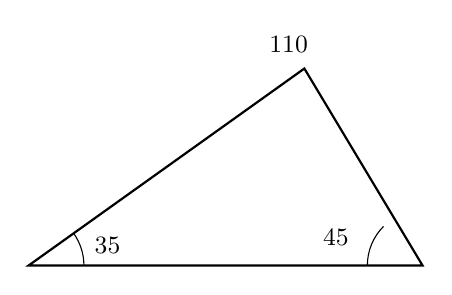
\begin{tikzpicture}[scale=1]
  \draw[thick] (0,0) -- (5,0) -- (3.5,2.5) -- cycle;
  \draw (0.7,0) arc[start angle=0,end angle=35,radius=0.7];
  \node at (1.0,0.25) {\small $35°$};
  \draw (4.3,0) arc[start angle=180,end angle=135,radius=0.7];
  \node at (3.9,0.35) {\small $45°$};
  \node at (3.3,2.8) {\small $110°$};
\end{tikzpicture}
\end{center}
\end{questionText}
\choiceA{Yes, because $35 + 45 + 110 = 190$}
\choiceB{Yes, because all angles are positive}
\choiceC{No, because the angles sum to $190°$ instead of $180°$}
\choiceD{No, because one angle is greater than $90°$}
\correctAnswer{C}
\explanation{$35 + 45 + 110 = 190 \neq 180$. Triangle angles must sum to exactly $180°$, so this triangle is not valid.}
\end{practiceQuestion}

\begin{practiceQuestion}{6-5-q07}{mc}
\begin{questionText}
A triangular prism is sliced with a cut parallel to its triangular base. What is the cross-section?
\end{questionText}
\choiceA{A rectangle}
\choiceB{A triangle congruent to the base}
\choiceC{A smaller triangle}
\choiceD{A trapezoid}
\correctAnswer{B}
\explanation{A cut parallel to the base of a prism always produces a shape congruent (same size and shape) to the base. For a triangular prism, this is a triangle identical to the base.}
\end{practiceQuestion}

\begin{practiceQuestion}{6-6-q28}{gmc}
\begin{questionText}
In the diagram, angle $1$ and angle $2$ are complementary. Angle $1$ measures $53°$. What is angle $2$?

\begin{center}
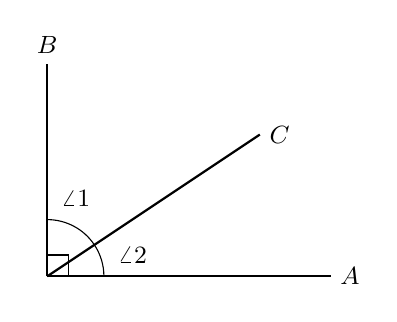
\begin{tikzpicture}[scale=0.9]
  \draw[thick] (0,0) -- (4,0);
  \draw[thick] (0,0) -- (0,3);
  \draw[thick] (0,0) -- (3,2);
  \draw (0.8,0) arc[start angle=0,end angle=34,radius=0.8];
  \node at (1.2,0.3) {\small $\angle 2$};
  \draw (0,0.8) arc[start angle=90,end angle=34,radius=0.8];
  \node at (0.4,1.1) {\small $\angle 1$};
  \node[right] at (4,0) {\small $A$};
  \node[above] at (0,3) {\small $B$};
  \node[right] at (3,2) {\small $C$};
  % Right angle mark
  \draw (0.3,0) -- (0.3,0.3) -- (0,0.3);
\end{tikzpicture}
\end{center}
\end{questionText}
\choiceA{$27°$}
\choiceB{$37°$}
\choiceC{$53°$}
\choiceD{$127°$}
\correctAnswer{B}
\explanation{The two angles together form a right angle ($90°$). $90° - 53° = 37°$.}
\end{practiceQuestion}

\begin{practiceQuestion}{7-3-q29}{gsa}
\begin{questionText}
The diagram shows a circular swimming pool. Find the area of the pool. Use $\pi \approx 3.14$.

\begin{center}
\begin{tikzpicture}[scale=0.4]
  \fill[cyan!20] (0,0) circle (3.5);
  \draw[thick,funBlue] (0,0) circle (3.5);
  \fill (0,0) circle (2pt) node[below] {center};
  \draw[thick,funRed,<->] (-3.5,0) -- (3.5,0);
  \node[above,funRed] at (0,0.2) {$18$ m};
\end{tikzpicture}
\end{center}
\end{questionText}
\correctAnswer{$254.34$ m$^2$}
\explanation{$r = 18 \div 2 = 9$ m. $A = \pi r^2 = 3.14 \times 81 = 254.34$ m$^2$.}
\end{practiceQuestion}

\begin{practiceQuestion}{7-4-q12}{mc}
\begin{questionText}
A square has sides of $10$ m. A quarter circle with radius $10$ m is removed from one corner. What is the area of the remaining figure? Use $\pi \approx 3.14$.
\end{questionText}
\choiceA{$21.5$ m$^2$}
\choiceB{$50$ m$^2$}
\choiceC{$78.5$ m$^2$}
\choiceD{$100$ m$^2$}
\correctAnswer{A}
\explanation{Square: $100$ m$^2$. Quarter circle: $\frac{1}{4} \times 3.14 \times 100 = 78.5$ m$^2$. Remaining: $100 - 78.5 = 21.5$ m$^2$.}
\end{practiceQuestion}

\begin{practiceQuestion}{7-5-q28}{gmc}
\begin{questionText}
The diagram shows a triangular prism. What is its total surface area?

\begin{center}
\begin{tikzpicture}[scale=0.4]
  % Front triangle
  \draw[thick,funBlue,fill=funBlue!10] (0,0) -- (6,0) -- (3,4) -- cycle;
  % Back triangle (offset)
  \draw[thick,funBlue,fill=funBlue!20] (2,1.5) -- (8,1.5) -- (5,5.5) -- cycle;
  % Connecting edges
  \draw[thick,funBlue] (0,0) -- (2,1.5);
  \draw[thick,funBlue] (6,0) -- (8,1.5);
  \draw[thick,funBlue] (3,4) -- (5,5.5);
  % Labels
  \node[below] at (3,0) {$6$ cm};
  \node[left] at (1.2,2) {$5$ cm};
  \node[right] at (4.8,2) {$5$ cm};
  \node[right] at (8,3.5) {$8$ cm};
  \node[above left] at (1,0.8) {$h = 4$ cm};
\end{tikzpicture}
\end{center}
\end{questionText}
\choiceA{$104$ cm$^2$}
\choiceB{$128$ cm$^2$}
\choiceC{$152$ cm$^2$}
\choiceD{$160$ cm$^2$}
\correctAnswer{C}
\explanation{Two triangles: $2 \times \frac{1}{2} \times 6 \times 4 = 24$ cm$^2$. Three rectangles: $6 \times 8 + 5 \times 8 + 5 \times 8 = 48 + 40 + 40 = 128$ cm$^2$. Total: $24 + 128 = 152$ cm$^2$.}
\end{practiceQuestion}

\begin{practiceQuestion}{7-6-q13}{mc}
\begin{questionText}
If you triple the height of a rectangular prism while keeping the base the same, what happens to the volume?
\end{questionText}
\choiceA{It stays the same}
\choiceB{It doubles}
\choiceC{It triples}
\choiceD{It increases by a factor of $9$}
\correctAnswer{C}
\explanation{$V = Bh$. If $h$ becomes $3h$, then $V = B(3h) = 3Bh$. The volume triples.}
\end{practiceQuestion}

\begin{practiceQuestion}{8-1-q10}{mc}
\begin{questionText}
Which question would require sampling rather than surveying the entire population?
\end{questionText}
\choiceA{How many students are in a classroom of $25$?}
\choiceB{What is the average lifespan of a light bulb produced by a factory?}
\choiceC{What is the total number of books on a shelf?}
\choiceD{How many chairs are in a room?}
\correctAnswer{B}
\explanation{Testing every light bulb would destroy them all. Sampling lets you estimate the average without testing every one.}
\end{practiceQuestion}

\begin{practiceQuestion}{8-3-q08}{mc}
\begin{questionText}
The dot plots for two classes overlap significantly. The difference in their means is $2$ points, and both have a MAD of $6$. What can you conclude?
\end{questionText}
\choiceA{The classes are very different}
\choiceB{The difference in means is meaningful}
\choiceC{The difference in means is small relative to the variability}
\choiceD{You cannot compare the classes}
\correctAnswer{C}
\explanation{The difference ($2$) is much smaller than the MAD ($6$), so the difference is not very meaningful — there is a lot of overlap.}
\end{practiceQuestion}

\begin{practiceQuestion}{8-4-q06}{mc}
\begin{questionText}
Team X: mean $82$, MAD $5$. Team Y: mean $76$, MAD $5$. Which team performed better on average, and is the difference meaningful?
\end{questionText}
\choiceA{Team X; no, because the difference is less than $2$ MADs}
\choiceB{Team X; yes, because $\frac{6}{5} = 1.2$ MADs, which is meaningful}
\choiceC{Team X; yes, because the means are more than $2$ MADs apart}
\choiceD{Team Y; yes, because its MAD is the same}
\correctAnswer{A}
\explanation{Difference $= 82 - 76 = 6$. In MADs: $\frac{6}{5} = 1.2$. Since $1.2 < 2$, the difference is not considered very meaningful.}
\end{practiceQuestion}

\begin{practiceQuestion}{8-6-q29}{gsa}
\begin{questionText}
The circle graph shows a family's monthly budget of $\$4{,}000$.

\begin{center}
\begin{tikzpicture}[scale=1.3]
  % Housing 35%, Food 20%, Transport 15%, Savings 10%, Other 20%
  % Angles: 126, 72, 54, 36, 72
  \fill[funBlue!50] (0,0) -- (90:1.5) arc (90:90-126:1.5) -- cycle;
  \fill[funGreen!50] (0,0) -- (90-126:1.5) arc (90-126:90-126-72:1.5) -- cycle;
  \fill[funOrange!50] (0,0) -- (90-126-72:1.5) arc (90-126-72:90-126-72-54:1.5) -- cycle;
  \fill[funRed!40] (0,0) -- (90-126-72-54:1.5) arc (90-126-72-54:90-126-72-54-36:1.5) -- cycle;
  \fill[gray!30] (0,0) -- (90-126-72-54-36:1.5) arc (90-126-72-54-36:90:1.5) -- cycle;
  \draw (0,0) circle (1.5);
  \node[font=\small\bfseries] at (27:1.05) {Housing};
  \node[font=\tiny] at (27:0.65) {$35\%$};
  \node[font=\small\bfseries] at (-62:1.05) {Food};
  \node[font=\tiny] at (-62:0.65) {$20\%$};
  \node[font=\small\bfseries] at (-125:1.05) {Transport};
  \node[font=\tiny] at (-125:0.65) {$15\%$};
  \node[font=\small\bfseries] at (-160:1.05) {Savings};
  \node[font=\tiny] at (-160:0.65) {$10\%$};
  \node[font=\small\bfseries] at (145:1.05) {Other};
  \node[font=\tiny] at (145:0.65) {$20\%$};
\end{tikzpicture}
\end{center}

How much money is spent on food? How much is saved?
\end{questionText}
\correctAnswer{Food: $\$800$; Savings: $\$400$}
\explanation{Food: $20\%$ of $\$4{,}000 = \$800$. Savings: $10\%$ of $\$4{,}000 = \$400$.}
\end{practiceQuestion}

\begin{practiceQuestion}{9-4-q13}{mc}
\begin{questionText}
A probability model has outcomes A, B, and C with $P(A) = 0.5$ and $P(B) = 0.3$. What is $P(C)$?
\end{questionText}
\choiceA{$0.8$}
\choiceB{$0.3$}
\choiceC{$0.2$}
\choiceD{$0.1$}
\correctAnswer{C}
\explanation{All probabilities must sum to $1$. $P(C) = 1 - 0.5 - 0.3 = 0.2$.}
\end{practiceQuestion}

\begin{practiceQuestion}{9-6-q09}{mc}
\begin{questionText}
A bag has $3$ red and $2$ blue marbles. You draw one marble, replace it, and draw again. What is the probability that both are red?
\end{questionText}
\choiceA{$\frac{6}{25}$}
\choiceB{$\frac{9}{25}$}
\choiceC{$\frac{3}{10}$}
\choiceD{$\frac{6}{20}$}
\correctAnswer{B}
\explanation{With replacement: $P = \frac{3}{5} \times \frac{3}{5} = \frac{9}{25}$.}
\end{practiceQuestion}

\begin{practiceQuestion}{9-7-q22}{sa}
\begin{questionText}
A simulation of $50$ coin flips produces $22$ heads. Predict how many heads you would expect in $200$ flips based on this simulation.
\end{questionText}
\correctAnswer{$88$}
\explanation{Experimental $P(\text{heads}) = \frac{22}{50} = 0.44$. In $200$ flips: $200 \times 0.44 = 88$.}
\end{practiceQuestion}
